%
% elltrigo.tex
%
% (c) 2022 Prof Dr Andreas Müller, OST Ostschweizer Fachhochschule
%

%
% elliptische Funktionen als Trigonometrie
%
\subsection{Elliptische Funktionen als Trigonometrie}
\begin{figure}
\centering
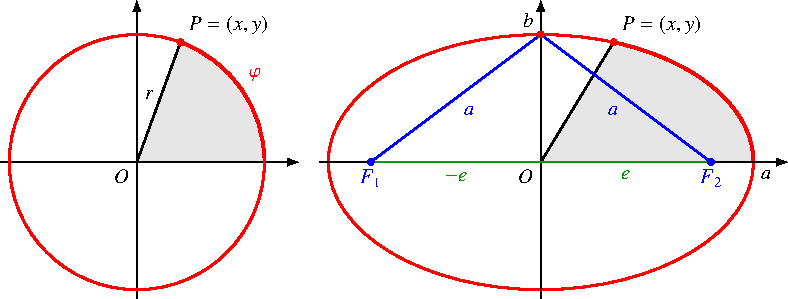
\includegraphics{chapters/110-elliptisch/images/ellipse.pdf}
\caption{Kreis und Ellipse zum Vergleich und zur Herleitung der 
elliptischen Funktionen von Jacobi als ``trigonometrische'' Funktionen
auf einer Ellipse.
\label{buch:elliptisch:fig:ellipse}}
\end{figure}
% based on Willliam Schwalm, Elliptic functions and elliptic integrals
% https://youtu.be/DCXItCajCyo

%
% Geometrie einer Ellipse
%
\subsubsection{Geometrie einer Ellipse}
Eine {\em Ellipse} ist die Menge der Punkte der Ebene, für die die Summe
\index{Ellipse}%
der Entfernungen von zwei festen Punkten $F_1$ und $F_2$,
den {\em Brennpunkten}, konstant ist.
\index{Brennpunkt}%
In Abbildung~\ref{buch:elliptisch:fig:ellipse} eine Ellipse
mit Brennpunkten in $F_1=(-e,0)$ und $F_2=(e,0)$ dargestellt,
die durch die Punkte $(\pm a,0)$ und $(0,\pm b)$ auf den Achsen geht.
Der Punkt $(a,0)$ hat die Entfernungen $a+e$ und $a-e$ von den beiden
Brennpunkten, also die Entfernungssumme $a+e+a-e=2a$.
Jeder andere Punkt auf der Ellipse muss ebenfalls diese Entfernungssumme
haben, insbesondere auch der Punkt $(0,b)$.
Seine Entfernung zu jedem Brennpunkt muss aus Symmetriegründen gleich gross,
also $a$ sein.
Aus dem Satz von Pythagoras liest man daher ab, dass
\[
b^2+e^2=a^2
\qquad\Rightarrow\qquad
e^2 = a^2-b^2
\]
sein muss.
Die Strecke $e$ heisst auch {\em (lineare) Exzentrizität} der Ellipse.
Das Verhältnis $\varepsilon= e/a$  heisst die {\em numerische Exzentrizität}
der Ellipse.

%
% Die Ellipsengleichung
%
\subsubsection{Ellipsengleichung}
Der Punkt $P=(x,y)$ auf der Ellipse hat die Entfernungen
\begin{equation}
\begin{aligned}
\overline{PF_1}^2
&=
y^2 + (x+e)^2
\\
\overline{PF_2}^2
&=
y^2 + (x-e)^2
\end{aligned}
\label{buch:elliptisch:eqn:wurzelausdruecke}
\end{equation}
von den Brennpunkten, für die 
\begin{equation}
\overline{PF_1}+\overline{PF_2}
=
2a
\label{buch:elliptisch:eqn:pf1pf2a}
\end{equation}
gelten muss.
Man kann nachrechnen, dass ein Punkt $P$, der die Gleichung
\[
\frac{x^2}{a^2} + \frac{y^2}{b^2}=1
\]
erfüllt, auch die Eigenschaft~\eqref{buch:elliptisch:eqn:pf1pf2a}
erfüllt.
Zur Vereinfachung setzen wir $l_1=\overline{PF_1}$ und $l_2=\overline{PF_2}$.
$l_1$ und $l_2$ sind Wurzeln aus der rechten Seite von
\eqref{buch:elliptisch:eqn:wurzelausdruecke}.
Das Quadrat von $l_1+l_2$ ist
\[
l_1^2 + 2l_1l_2 + l_2^2 = 4a^2.
\]
Um die Wurzeln ganz zu eliminieren, bringt man das Produkt $l_1l_2$ alleine
auf die rechte Seite und quadriert.
Man muss also verifizieren, dass
\[
(l_1^2 + l_2^2 -4a^2)^2 = 4l_1^2l_2^2.
\]
In den entstehenden Ausdrücken muss man ausserdem $e=\sqrt{a^2-b^2}$ und
\[
y=b\sqrt{1-\frac{x^2}{a^2}}
\]
substituieren.
Diese Rechnung führt man am einfachsten mit Hilfe eines
Computeralgebraprogramms durch, welches obige Behauptung bestätigt.

%
% Normierung
%
\subsubsection{Normierung}
Die trigonometrischen Funktionen sind definiert als Verhältnisse 
von Seiten rechtwinkliger Dreiecke.
Dadurch, dass man den die Hypothenuse auf Länge $1$ normiert, 
kann man die Sinus- und Kosinus-Funktion als Koordinaten eines
Punktes auf dem Einheitskreis interpretieren.

Für die Koordinaten eines Punktes auf der Ellipse ist dies nicht so einfach,
weil es nicht nur eine Ellipse gibt, sondern für jede numerische Exzentrizität
mindestens eine mit Halbeachse $1$.
Wir wählen die Ellipsen so, dass $a$ die grosse Halbachse ist, also $a>b$.
Als Normierungsbedingung verwenden wir, dass $b=1$ sein soll, wie in
Abbildung~\ref{buch:elliptisch:fig:jacobidef}.
Dann ist $a=1/\varepsilon>1$.
In dieser Normierung haben Punkte $(x,y)$ auf der Ellipse $y$-Koordinaten
zwischen $-1$ und $1$ und $x$-Koordinaten zwischen $-a$ und $a$.

Im Zusammenhang mit elliptischen Funktionen wird die numerische Exzentrizität
$\varepsilon$ auch mit
\[
k
=
\varepsilon
=
\frac{e}{a}
=
\frac{\sqrt{a^2-b^2}}{a}
=
\frac{\sqrt{a^2-1}}{a},
\]
die Zahl $k$ heisst auch der {\em Modulus}.
Man kann $a$ auch durch $k$ ausdrücken, durch Quadrieren und Umstellen
findet man
\[
k^2a^2 = a^2-1
\quad\Rightarrow\quad
1=a^2(k^2-1)
\quad\Rightarrow\quad
a=\frac{1}{\sqrt{k^2-1}}.
\]

Die Gleichung der ``Einheitsellipse'' zu diesem Modulus ist
\[
\frac{x^2}{a^2}+y^2=1
\qquad\text{oder}\qquad
x^2(k^2-1) + y^2 = 1.
\]

%
% Definition der elliptischen Funktionen
%
\begin{figure}
\centering
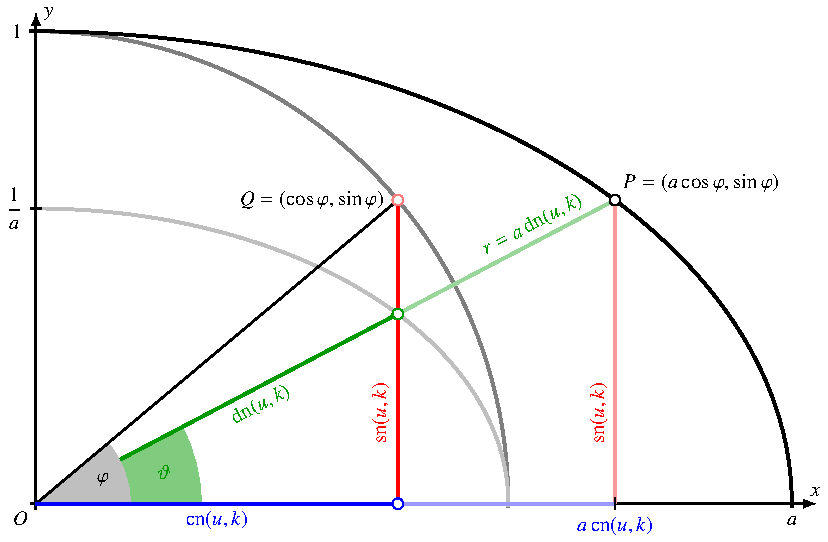
\includegraphics{chapters/110-elliptisch/images/jacobidef.pdf}
\caption{Definition der elliptischen Funktionen als Trigonometrie
an einer Ellipse mit Halbachsen $a$ und $1$.
\label{buch:elliptisch:fig:jacobidef}}
\end{figure}
\subsubsection{Definition der elliptischen Funktionen}
Die elliptischen Funktionen für einen Punkt $P$ auf der Ellipse mit Modulus $k$
können jetzt als Verhältnisse der Koordinaten des Punktes definieren.
Es stellt sich aber die Frage, was man als Argument verwenden soll.
Es soll so etwas wie den Winkel $\varphi$ zwischen der $x$-Achse und dem
Radiusvektor zum Punkt $P$
darstellen, aber wir haben hier noch eine Wahlfreiheit, die wir später
ausnützen möchten.
Im Moment müssen wir die Frage noch nicht beantworten und nennen das
noch unbestimmte Argument $u$.
Wir kümmern uns später um die Frage, wie $u$ von $\varphi$ abhängt.

Die Funktionen, die wir definieren wollen, hängen ausserdem auch 
vom Modulus ab.
Falls der verwendete Modulus aus dem Zusammenhang klar ist, lassen
wir das $k$-Argument weg.

Die Punkte auf dem Einheitskreis haben alle den gleichen Abstand vom
Nullpunkt, dies ist gleichzeitig die definierende Gleichung $r^2=x^2+y^2=1$
des Kreises.
Die Punkte auf der Ellipse erfüllen die Gleichung $x^2/a^2+y^2=1$,
die Entfernung der Punkte $r=\sqrt{x^2+y^2}$ vom Nullpunkt variert aber.

In Analogie zu den trigonometrischen Funktionen setzen wir jetzt für 
die Funktionen
\[
\begin{aligned}
&\text{sinus amplitudinis:}&
{\color{red}\operatorname{sn}(u,k)}&= y \\
&\text{cosinus amplitudinis:}&
{\color{blue}\operatorname{cn}(u,k)}&= \frac{x}{a} \\
&\text{delta amplitudinis:}&
{\color{darkgreen}\operatorname{dn}(u,k)}&=\frac{r}{a},
\end{aligned}
\]
die auch in Abbildung~\ref{buch:elliptisch:fig:jacobidef}
dargestellt sind.
Aus der Gleichung der Ellipse folgt sofort, dass
\[
\operatorname{sn}(u,k)^2 + \operatorname{cn}(u,k)^2 = 1
\]
ist.
Der Satz von Pythagoras kann verwendet werden, um die Entfernung zu
berechnen, also gilt
\begin{equation}
r^2
=
a^2 \operatorname{dn}(u,k)^2
=
x^2 + y^2
=
a^2\operatorname{cn}(u,k)^2 + \operatorname{sn}(u,k)^2
\quad
\Rightarrow
\quad
a^2 \operatorname{dn}(u,k)^2
=
a^2\operatorname{cn}(u,k)^2 + \operatorname{sn}(u,k)^2.
\label{buch:elliptisch:eqn:sncndnrelation}
\end{equation}
Ersetzt man
$
a^2\operatorname{cn}(u,k)^2
=
a^2-a^2\operatorname{sn}(u,k)^2
$, ergibt sich
\[
a^2 \operatorname{dn}(u,k)^2
=
a^2-a^2\operatorname{sn}(u,k)^2
+
\operatorname{sn}(u,k)^2
\quad
\Rightarrow
\quad
\operatorname{dn}(u,k)^2
+
\frac{a^2-1}{a^2}\operatorname{sn}(u,k)^2
=
1,
\]
woraus sich die Identität
\[
\operatorname{dn}(u,k)^2 + k^2 \operatorname{sn}(u,k)^2 = 1
\]
ergibt.
Ebenso kann man aus~\eqref{buch:elliptisch:eqn:sncndnrelation}
die Funktion $\operatorname{cn}(u,k)$ eliminieren, was auf
\[
a^2\operatorname{dn}(u,k)^2
=
a^2\operatorname{cn}(u,k)^2
+1-\operatorname{cn}(u,k)^2
=
(a^2-1)\operatorname{cn}(u,k)^2
+1.
\]
Nach Division durch $a^2$ ergibt sich
\begin{align*}
\operatorname{dn}(u,k)^2
-
k^2\operatorname{cn}(u,k)^2
&=
\frac{1}{a^2}
=
\frac{a^2-a^2+1}{a^2}
=
1-k^2 =: k^{\prime 2}.
\end{align*}
Wir stellen die hiermit gefundenen Relationen zwischen den grundlegenden
Jacobischen elliptischen Funktionen für später zusammen in den Formeln
\begin{equation}
\begin{aligned}
\operatorname{sn}^2(u,k)
+
\operatorname{cn}^2(u,k)
&=
1
\\
\operatorname{dn}^2(u,k) + k^2\operatorname{sn}^2(u,k)
&=
1
\\
\operatorname{dn}^2(u,k)  -k^2\operatorname{cn}^2(u,k)
&=
k^{\prime 2}.
\end{aligned}
\label{buch:elliptisch:eqn:jacobi-relationen}
\end{equation}
zusammen.
So wie es möglich ist, $\sin\alpha$ durch $\cos\alpha$ auszudrücken,
ist es mit
\eqref{buch:elliptisch:eqn:jacobi-relationen}
jetzt auch möglich jede grundlegende elliptische Funktion durch
jede anderen auszudrücken.
Die Resultate sind in der Tabelle~\ref{buch:elliptisch:fig:jacobi-relationen}
zusammengestellt.

\begin{table}
\centering
\renewcommand{\arraystretch}{2.1}
\begin{tabular}{|>{$\displaystyle}c<{$}|>{$\displaystyle}c<{$}>{$\displaystyle}c<{$}>{$\displaystyle}c<{$}|}
\hline
&\operatorname{sn}(u,k)
&\operatorname{cn}(u,k)
&\operatorname{dn}(u,k)\\
\hline
\operatorname{sn}(u,k)
&\operatorname{sn}(u,k)
&\sqrt{1-\operatorname{cn}^2(u,k)}
&\frac1k\sqrt{1-\operatorname{dn}^2(u,k)}
\\
\operatorname{cn}(u,k)
&\sqrt{1-\operatorname{sn}^2(u,k)}
&\operatorname{cn}(u,k)
&\frac{1}{k}\sqrt{\operatorname{dn}^2(u,k)-k^{\prime2}}
\\
\operatorname{dn}(u,k)
&\sqrt{1-k^2\operatorname{sn}^2(u,k)}
&\sqrt{k^{\prime2}+k^2\operatorname{cn}^2(u,k)}
&\operatorname{dn}(u,k)
\\
\hline
\end{tabular}
\caption{Jede der Jacobischen elliptischen Funktionen lässt sich
unter Verwendung der Relationen~\eqref{buch:elliptisch:eqn:jacobi-relationen}
durch jede andere ausdrücken.
\label{buch:elliptisch:fig:jacobi-relationen}}
\end{table}

%
% Ableitungen der Jacobi-ellpitischen Funktionen
% 
\subsubsection{Ableitung}
Die trigonometrischen Funktionen sind deshalb so besonders nützlich 
für die Lösung von Schwingungsdifferentialgleichungen, weil sie die
Beziehungen
\[
\frac{d}{d\varphi}  \cos\varphi = -\sin\varphi
\qquad\text{und}\qquad
\frac{d}{d\varphi}  \sin\varphi = \cos\varphi
\]
erfüllen.
So einfach können die Beziehungen natürlich nicht sein, sonst würde sich
durch Integration ja wieder nur die trigonometrischen Funktionen ergeben.
Durch geschickte Wahl des Arguments $u$ kann man aber erreichen, dass
sie ähnlich nützliche Beziehungen zwischen den Ableitungen ergeben.

Gesucht ist jetzt also eine Wahl für das Argument $u$ zum Beispiel in
Abhängigkeit von $\varphi$, dass sich einfache und nützliche
Ableitungsformeln ergeben.
Wir setzen daher $u(\varphi)$ voraus und beachten, dass $x$ und $y$
ebenfalls von $\varphi$ abhängen, es ist
$y=\sin\varphi$ und $x=a\cos\varphi$.
Die Ableitungen von $x$ und $y$ nach $\varphi$ sind
\begin{align*}
\frac{dy}{d\varphi}
&=
\cos\varphi
=
\frac{1}{a} x
=
\operatorname{cn}(u,k)
\\
\frac{dx}{d\varphi}
&=
-a\sin\varphi
=
-a y
=
-a\operatorname{sn}(u,k).
\end{align*}
Daraus kann man jetzt die folgenden Ausdrücke für die Ableitungen der
elliptischen Funktionen nach $\varphi$ ableiten:
\begin{align*}
\frac{d}{d\varphi} \operatorname{sn}(u,z)
&=
\frac{d}{d\varphi} y(\varphi)
=
\cos\varphi
=
\frac{x}{a}
=
\operatorname{cn}(u,k)
&&\Rightarrow&
\frac{d}{du}
\operatorname{sn}(u,k)
&=
\operatorname{cn}(u,k) \frac{d\varphi}{du}
\\
\frac{d}{d\varphi} \operatorname{cn}(u,z)
&=
\frac{d}{d\varphi} \frac{x(\varphi)}{a}
=
-\sin\varphi
=
-\operatorname{sn}(u,k)
&&\Rightarrow&
\frac{d}{du}\operatorname{cn}(u,k)
&=
-\operatorname{sn}(u,k) \frac{d\varphi}{du}
\\
\frac{d}{d\varphi} \operatorname{dn}(u,z)
&=
\frac{1}{a}\frac{dr}{d\varphi}
=
\frac{1}{a}\frac{d\sqrt{x^2+y^2}}{d\varphi}
%\\
%&
\rlap{$\displaystyle\mathstrut
=
\frac{x}{ar} \frac{dx}{d\varphi}
+
\frac{y}{ar} \frac{dy}{d\varphi}
%\\
%&
=
\frac{x}{ar} (-a\operatorname{sn}(u,k))
+
\frac{y}{ar} \operatorname{cn}(u,k)
$}
\\
&
\rlap{$\displaystyle\mathstrut
=
\frac{x}{ar}(-ay)
+
\frac{y}{ar} \frac{x}{a}
%\rlap{$\displaystyle
=
\frac{xy(-1+\frac{1}{a^2})}{r} 
%$}
%\\
%&
=
-\frac{xy(a^2-1)}{a^2r} 
$}
\\
&=
-\frac{a^2-1}{ar}
\operatorname{cn}(u,k) \operatorname{sn}(u,k)
%\\
%&
\rlap{$\displaystyle\mathstrut
=
-k^2
\frac{a}{r}
\operatorname{cn}(u,k) \operatorname{sn}(u,k)
$}
\\
&=
-k^2\frac{\operatorname{cn}(u,k)\operatorname{sn}(u,k)}{\operatorname{dn}(u,k)}
&&\Rightarrow&
\frac{d}{du} \operatorname{dn}(u,k)
&=
-k^2\frac{\operatorname{cn}(u,k)
\operatorname{sn}(u,k)}{\operatorname{dn}(u,k)}
\frac{d\varphi}{du}.
\end{align*}
Die einfachsten Beziehungen ergeben sich offenbar, wenn man $u$ so
wählt, dass
\[
\frac{d\varphi}{du}
=
\operatorname{dn}(u,k)
=
\frac{r}{a}.
\]
Damit haben wir die grundlegenden Ableitungsregeln

\begin{satz}
\label{buch:elliptisch:satz:ableitungen}
Die Jacobischen elliptischen Funktionen haben die Ableitungen
\begin{equation}
\begin{aligned}
\frac{d}{du}\operatorname{sn}(u,k)
&=
\phantom{-}\operatorname{cn}(u,k)\operatorname{dn}(u,k)
\\
\frac{d}{du}\operatorname{cn}(u,k)
&=
-\operatorname{sn}(u,k)\operatorname{dn}(u,k)
\\
\frac{d}{du}\operatorname{dn}(u,k)
&=
-k^2\operatorname{sn}(u,k)\operatorname{cn}(u,k).
\end{aligned}
\label{buch:elliptisch:eqn:ableitungsregeln}
\end{equation}
\end{satz}

%
% Der Grenzfall $k=1$
%
\subsubsection{Der Grenzwert $k\to1$}
\begin{figure}
\centering
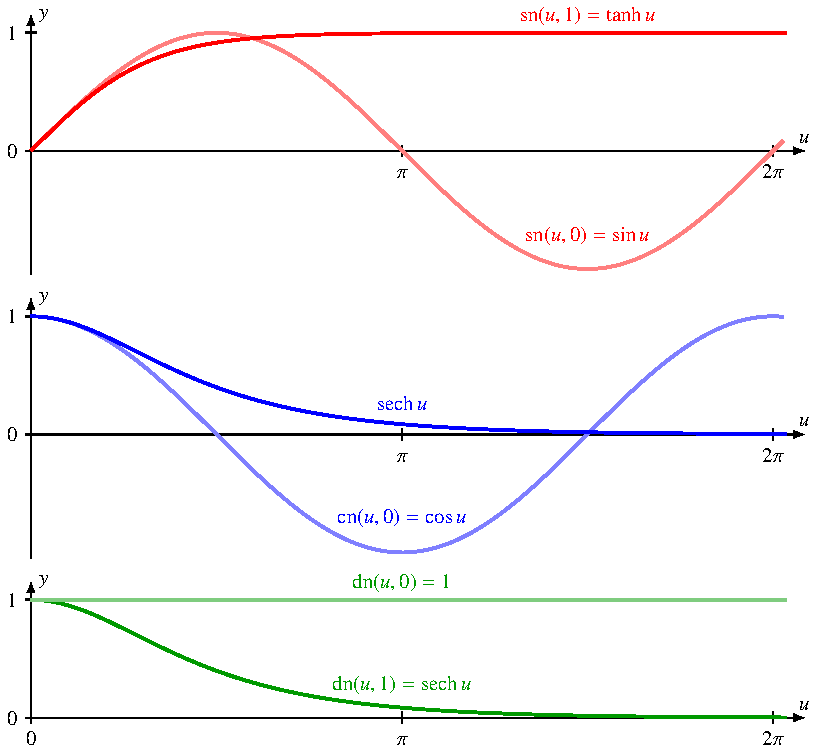
\includegraphics{chapters/110-elliptisch/images/sncnlimit.pdf}
\caption{Grenzfälle der Jacobischen elliptischen Funktionen 
für die Werte $0$ und $1$ des Parameters $k$.
\label{buch:elliptisch:fig:sncnlimit}}
\end{figure}
Für $k=1$ ist $k^{\prime2}=1-k^2=$ und es folgt aus den
Relationen~\eqref{buch:elliptisch:eqn:jacobi-relationen}
\[
\operatorname{cn}^2(u,k)
-
k^2
\operatorname{dn}^2(u,k)
=
k^{\prime2}
=
0
\qquad\Rightarrow\qquad
\operatorname{cn}^2(u,1)
=
\operatorname{dn}^2(u,1),
\]
die beiden Funktionen
$\operatorname{cn}(u,k)$
und
$\operatorname{dn}(u,k)$
fallen also zusammen.
Die Ableitungsregeln werden dadurch vereinfacht:
\begin{align*}
\operatorname{sn}'(u,1)
&=
\operatorname{cn}(u,1)
\operatorname{dn}(u,1)
=
\operatorname{cn}^2(u,1)
=
1-\operatorname{sn}^2(u,1)
&&\Rightarrow& y'&=1-y^2
\\
\operatorname{cn}'(u,1)
&=
-
\operatorname{sn}(u,1)
\operatorname{dn}(u,1)
=
-
\operatorname{sn}(u,1)\operatorname{cn}(u,1)
&&\Rightarrow&
\frac{z'}{z}&=(\log z)' = -y
\end{align*}
Die erste Differentialgleichung für $y$ lässt sich separieren, man findet
die Lösung
\[
\frac{y'}{1-y^2}
=
1
\quad\Rightarrow\quad
\int \frac{dy}{1-y^2} = \int \,du
\quad\Rightarrow\quad
\operatorname{artanh}(y) = u
\quad\Rightarrow\quad
\operatorname{sn}(u,1)=\tanh u.
\]
Damit kann man jetzt auch $z$ berechnen:
\begin{align*}
(\log \operatorname{cn}(u,1))'
&=
\tanh u
&&\Rightarrow&
\log\operatorname{cn}(u,1)
&=
-\int\tanh u\,du
=
-\log\cosh u
\\
&
&&\Rightarrow&
\operatorname{cn}(u,1)
&=
\frac{1}{\cosh u}
=
\operatorname{sech}u.
\end{align*}
Die Grenzfunktionen sind in Abbildung~\ref{buch:elliptisch:fig:sncnlimit}
dargestellt.

%
% Das Argument u
%
\subsubsection{Das Argument $u$}
Die Gleichung 
\begin{equation}
\frac{d\varphi}{du}
=
\operatorname{dn}(u,k)
\label{buch:elliptisch:eqn:uableitung}
\end{equation}
ermöglicht, $\varphi$ in Abhängigkeit von $u$ zu berechnen, ohne jedoch
die geometrische Bedeutung zu klären.
Das beginnt bereits damit, dass der Winkel $\varphi$ nicht nicht der
Polarwinkel des Punktes $P$ in Abbildung~\ref{buch:elliptisch:fig:jacobidef}
ist, diesen nennen wir $\vartheta$.
Der Zusammenhang zwischen $\varphi$ und $\vartheta$ ist
\begin{equation}
\frac1{a}\tan\varphi = \tan\vartheta
\label{buch:elliptisch:eqn:phitheta}
\end{equation}

Um die geometrische Bedeutung besser zu verstehen, nehmen wir jetzt an,
dass die Ellipse mit einem Parameter $t$ parametrisiert ist, dass also
$\varphi(t)$, $\vartheta(t)$ und $u(t)$ Funktionen von $t$ sind.
Die Ableitung von~\eqref{buch:elliptisch:eqn:phitheta} ist
\[
\frac1{a}\cdot \frac{1}{\cos^2\varphi}\cdot \dot{\varphi}
=
\frac{1}{\cos^2\vartheta}\cdot \dot{\vartheta}.
\]
Daraus kann die Ableitung von $\vartheta$ nach $\varphi$ bestimmt
werden, sie ist
\[
\frac{d\vartheta}{d\varphi}
=
\frac{\dot{\vartheta}}{\dot{\varphi}}
=
\frac{1}{a}
\cdot
\frac{\cos^2\vartheta}{\cos^2\varphi}
=
\frac{1}{a}
\cdot
\frac{(x/r)^2}{(x/a)^2}
=
\frac{1}{a}\cdot
\frac{a^2}{r^2}
=
\frac{1}{a}\cdot\frac{1}{\operatorname{dn}^2(u,k)}.
\]
Damit kann man jetzt mit Hilfe von~\eqref{buch:elliptisch:eqn:uableitung} 
Die Ableitung von $\vartheta$ nach $u$ ermitteln, sie ist
\[
\frac{d\vartheta}{du}
=
\frac{d\vartheta}{d\varphi}
\cdot
\frac{d\varphi}{du}
=
\frac{1}{a}\cdot\frac{1}{\operatorname{dn}^2(u,k)}
\cdot
\operatorname{dn}(u,k)
=
\frac{1}{a}
\cdot
\frac{1}{\operatorname{dn}(u,k)}
=
\frac{1}{a}
\cdot\frac{a}{r}
=
\frac{1}{r},
\]
wobei wir auch die Definition der Funktion $\operatorname{dn}(u,k)$
verwendet haben.

In der Parametrisierung mit dem Parameter $t$ kann man jetzt die Ableitung
von $u$ nach $t$ berechnen als
\[
\frac{du}{dt}
=
\frac{du}{d\vartheta}
\frac{d\vartheta}{dt}
=
r
\dot{\vartheta}.
\]
Darin ist $\dot{\vartheta}$ die Winkelgeschwindigkeit des Punktes um
das Zentrum $O$ und $r$ ist die aktuelle Entfernung des Punktes $P$
von $O$.
$r\dot{\vartheta}$ ist also die Geschwindigkeitskomponenten des Punktes
$P$ senkrecht auf den aktuellen Radiusvektor.
Der Parameter $u$, der zum Punkt $P$ gehört, ist also das Integral
\[
u(P) = \int_0^P r\,d\vartheta.
\]
Für einen Kreis ist die Geschwindigkeit von $P$ immer senkrecht
auf dem Radiusvektor und der Radius ist konstant, so dass
$u(P)=\vartheta(P)$ ist.

%
% Die abgeleiteten elliptischen Funktionen
%
\begin{figure}
\centering
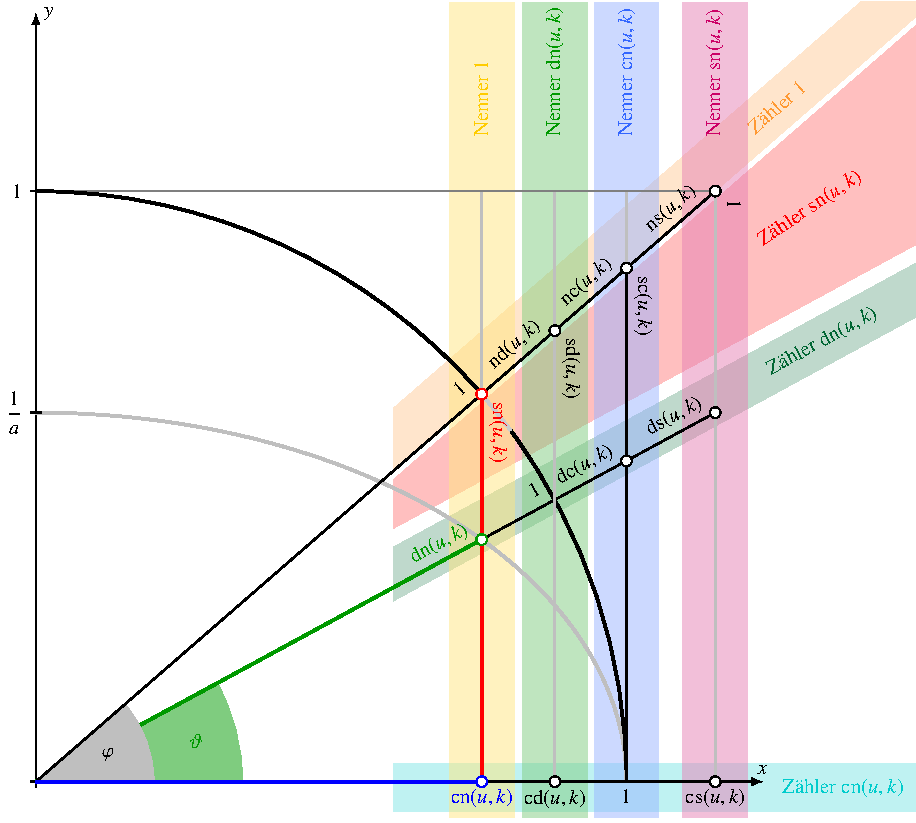
\includegraphics[width=\textwidth]{chapters/110-elliptisch/images/jacobi12.pdf}
\caption{Die Verhältnisse der Funktionen
$\operatorname{sn}(u,k)$,
$\operatorname{cn}(u,k)$
udn
$\operatorname{dn}(u,k)$
geben Anlass zu neun weitere Funktionen, die sich mit Hilfe
des Strahlensatzes geometrisch interpretieren lassen.
\label{buch:elliptisch:fig:jacobi12}}
\end{figure}
\begin{table}
\centering
\renewcommand{\arraystretch}{2.5}
\begin{tabular}{|>{$\displaystyle}c<{$}|>{$\displaystyle}c<{$}>{$\displaystyle}c<{$}>{$\displaystyle}c<{$}>{$\displaystyle}c<{$}|}
\hline
\cdot &
\frac{1}{1} &
\frac{1}{\operatorname{sn}(u,k)} &
\frac{1}{\operatorname{cn}(u,k)} &
\frac{1}{\operatorname{dn}(u,k)} 
\\[5pt]
\hline
1&
&%\operatorname{nn}(u,k)=\frac{1}{1} &
\operatorname{ns}(u,k)=\frac{1}{\operatorname{sn}(u,k)} &
\operatorname{nc}(u,k)=\frac{1}{\operatorname{cn}(u,k)} &
\operatorname{nd}(u,k)=\frac{1}{\operatorname{dn}(u,k)}
\\
\operatorname{sn}(u,k) &
\operatorname{sn}(u,k)=\frac{\operatorname{sn}(u,k)}{1}&
&%\operatorname{ss}(u,k)=\frac{\operatorname{sn}(u,k)}{\operatorname{sn}(u,k)}&
\operatorname{sc}(u,k)=\frac{\operatorname{sn}(u,k)}{\operatorname{cn}(u,k)}&
\operatorname{sd}(u,k)=\frac{\operatorname{sn}(u,k)}{\operatorname{dn}(u,k)}
\\
\operatorname{cn}(u,k) &
\operatorname{cn}(u,k)=\frac{\operatorname{cn}(u,k)}{1} &
\operatorname{cs}(u,k)=\frac{\operatorname{cn}(u,k)}{\operatorname{sn}(u,k)}&
&%\operatorname{cc}(u,k)=\frac{\operatorname{cn}(u,k)}{\operatorname{cn}(u,k)}&
\operatorname{cd}(u,k)=\frac{\operatorname{cn}(u,k)}{\operatorname{dn}(u,k)}
\\
\operatorname{dn}(u,k) &
\operatorname{dn}(u,k)=\frac{\operatorname{dn}(u,k)}{1} &
\operatorname{ds}(u,k)=\frac{\operatorname{dn}(u,k)}{\operatorname{sn}(u,k)}&
\operatorname{dc}(u,k)=\frac{\operatorname{dn}(u,k)}{\operatorname{cn}(u,k)}&
%\operatorname{dd}(u,k)=\frac{\operatorname{dn}(u,k)}{\operatorname{dn}(u,k)}
\\[5pt]
\hline
\end{tabular}
\caption{Zusammenstellung der abgeleiteten Jacobischen elliptischen
Funktionen in hinteren drei Spalten als Quotienten der grundlegenden
Jacobischen elliptischen Funktionen.
Die erste Spalte zum Nenner $1$ enthält die grundlegenden
Jacobischen elliptischen Funktionen.
\label{buch:elliptisch:table:abgeleitetjacobi}}
\end{table}

%
% Die abgeleiteten elliptischen Funktionen
%
\subsubsection{Die abgeleiteten elliptischen Funktionen}
Zusätzlich zu den grundlegenden Jacobischen elliptischen Funktioenn
lassen sich weitere elliptische Funktionen bilden, die unglücklicherweise
die {\em abgeleiteten elliptischen Funktionen} genannt werden.
Ähnlich wie die trigonometrischen Funktionen $\tan\alpha$, $\cot\alpha$,
$\sec\alpha$ und $\csc\alpha$ als Quotienten von $\sin\alpha$ und
$\cos\alpha$ definiert sind, sind die abgeleiteten elliptischen Funktionen
die in Tabelle~\ref{buch:elliptisch:table:abgeleitetjacobi} zusammengestellten
Quotienten der grundlegenden Jacobischen elliptischen Funktionen.
Die Bezeichnungskonvention ist, dass die Funktion $\operatorname{pq}(u,k)$
ein Quotient ist, dessen Zähler durch den Buchstaben p bestimmt ist,
der Nenner durch den Buchstaben q.
Der Buchstabe n steht für eine $1$, die Buchstaben s, c und d stehen für
die Anfangsbuchstaben der grundlegenden Jacobischen elliptischen
Funktionen.
Meint man irgend eine der Jacobischen elliptischen Funktionen, schreibt
man manchmal auch $\operatorname{zn}(u,k)$.

In Abbildung~\ref{buch:elliptisch:fig:jacobi12} sind die Quotienten auch
geometrisch interpretiert.
Der Wert der Funktion $\operatorname{nq}(u,k)$ ist die auf dem Strahl
mit Polarwinkel $\varphi$ abgetragene Länge bis zu den vertikalen
Geraden, die den verschiedenen möglichen Nennern entsprechen.
Entsprechend ist der Wert der Funktion $\operatorname{dq}(u,k)$ die
Länge auf dem Strahl mit Polarwinkel $\vartheta$.

Die Relationen~\ref{buch:elliptisch:eqn:jacobi-relationen}
ermöglichen, jede Funktion $\operatorname{zn}(u,k)$ durch jede
andere auszudrücken.
Die schiere Anzahl solcher Beziehungen macht es unmöglich, sie 
übersichtlich in einer Tabelle zusammenzustellen, daher soll hier
nur an einem Beispiel das Vorgehen gezeigt werden:

\begin{beispiel}
Die Funktion $\operatorname{sc}(u,k)$ soll durch $\operatorname{cd}(u,k)$
ausgedrückt werden.
Zunächst ist 
\[
\operatorname{sc}(u,k)
=
\frac{\operatorname{sn}(u,k)}{\operatorname{cn}(u,k)}
\]
nach Definition.
Im Resultat sollen nur noch $\operatorname{cn}(u,k)$ und
$\operatorname{dn}(u,k)$ vorkommen.
Daher eliminieren wir zunächst die Funktion $\operatorname{sn}(u,k)$
mit Hilfe von \eqref{buch:elliptisch:eqn:jacobi-relationen} und erhalten
\begin{equation}
\operatorname{sc}(u,k)
=
\frac{\sqrt{1-\operatorname{cn}^2(u,k)}}{\operatorname{cn}(u,k)}.
\label{buch:elliptisch:eqn:allgausdruecken}
\end{equation}
Nun genügt es, die Funktion $\operatorname{cn}(u,k)$ durch
$\operatorname{cd}(u,k)$ auszudrücken.
Aus der Definition und der
dritten Relation in \eqref{buch:elliptisch:eqn:jacobi-relationen} 
erhält man
\begin{align*}
\operatorname{cd}^2(u,k)
&=
\frac{\operatorname{cn}^2(u,k)}{\operatorname{dn}^2(u,k)}
=
\frac{\operatorname{cn}^2(u,k)}{k^{\prime2}+k^2\operatorname{cn}^2(u,k)}
\\
\Rightarrow
\qquad
k^{\prime 2}
\operatorname{cd}^2(u,k)
+
k^2\operatorname{cd}^2(u,k)\operatorname{cn}^2(u,k)
&=
\operatorname{cn}^2(u,k)
\\
\operatorname{cn}^2(u,k)
-
k^2\operatorname{cd}^2(u,k)\operatorname{cn}^2(u,k)
&=
k^{\prime 2}
\operatorname{cd}^2(u,k)
\\
\operatorname{cn}^2(u,k)
&=
\frac{
k^{\prime 2}
\operatorname{cd}^2(u,k)
}{
1 - k^2\operatorname{cd}^2(u,k)
}
\end{align*}
Für den Zähler brauchen wir $1-\operatorname{cn}^2(u,k)$, also
\[
1-\operatorname{cn}^2(u,k)
=
\frac{
1
-
k^2\operatorname{cd}^2(u,k)
-
k^{\prime 2}
\operatorname{cd}^2(u,k)
}{
1
-
k^2\operatorname{cd}^2(u,k)
}
=
\frac{1-\operatorname{cd}^2(u,k)}{1-k^2\operatorname{cd}^2(u,k)}
\]
Einsetzen in~\eqref{buch:elliptisch:eqn:allgausdruecken} gibt
\begin{align*}
\operatorname{sc}(u,k)
&=
\frac{
\sqrt{1-\operatorname{cd}^2(u,k)}
}{\sqrt{1-k^2\operatorname{cd}^2(u,k)}}
\cdot
\frac{
\sqrt{1 - k^2\operatorname{cd}^2(u,k)}
}{
k'
\operatorname{cd}(u,k)
}
=
\frac{
\sqrt{1-\operatorname{cd}^2(u,k)}
}{
k'
\operatorname{cd}(u,k)
}.
\qedhere
\end{align*}
\end{beispiel}

\subsubsection{Ableitung der abgeleiteten elliptischen Funktionen}
Aus den Ableitungen der grundlegenden Jacobischen elliptischen Funktionen
können mit der Quotientenregel nun auch beliebige Ableitungen der
abgeleiteten Jacobischen elliptischen Funktionen gefunden werden.
Als Beispiel berechnen wir die Ableitung von $\operatorname{sc}(u,k)$.
Sie ist
\begin{align*}
\frac{d}{du}
\operatorname{sc}(u,k)
&=
\frac{d}{du}
\frac{\operatorname{sn}(u,k)}{\operatorname{cn}(u,k)}
=
\frac{
\operatorname{sn}'(u,k)\operatorname{cn}(u,k)
-
\operatorname{sn}(u,k)\operatorname{cn}'(u,k)}{
\operatorname{cn}^2(u,k)
}
\\
&=
\frac{
\operatorname{cn}^2(u,k)\operatorname{dn}(u,k)
+
\operatorname{sn}^2(u,k)\operatorname{dn}(u,k)
}{
\operatorname{cn}^2(u,k)
}
=
\frac{(
\operatorname{sn}^2(u,k)
+
\operatorname{cn}^2(u,k)
)\operatorname{dn}(u,k)}{
\operatorname{cn}^2(u,k)
}
\\
&=
\frac{1}{\operatorname{cn}(u,k)}
\cdot
\frac{\operatorname{dn}(u,k)}{\operatorname{cn}(u,k)}
=
\operatorname{nc}(u,k)
\operatorname{dc}(u,k).
\end{align*}
Man beachte, dass das Quadrat der Nennerfunktion im Resultat
der Quotientenregel zur Folge hat, dass die
beiden Funktionen im Resultat beide den gleichen Nenner haben wie
die Funktion, die abgeleitet wird.

Mit etwas Fleiss kann man nach diesem Muster alle Ableitungen
\begin{equation}
%\small
\begin{aligned}
\operatorname{sn}'(u,k)
&= 
\phantom{-}
\operatorname{cn}(u,k)\,\operatorname{dn}(u,k)
&&\qquad&
\operatorname{ns}'(u,k)
&=
-
\operatorname{cs}(u,k)\,\operatorname{ds}(u,k)
\\
\operatorname{cn}'(u,k)
&= 
-
\operatorname{sn}(u,k)\,\operatorname{dn}(u,k)
&&&
\operatorname{nc}'(u,k)
&=
\phantom{-}
\operatorname{sc}(u,k)\,\operatorname{dc}(u,k)
\\
\operatorname{dn}'(u,k)
&= 
-k^2
\operatorname{sn}(u,k)\,\operatorname{cn}(u,k)
&&&
\operatorname{nd}'(u,k)
&=
\phantom{-}
k^2
\operatorname{sd}(u,k)\,\operatorname{cd}(u,k)
\\
\operatorname{sc}'(u,k)
&=
\phantom{-}
\operatorname{dc}(u,k)\,\operatorname{nc}(u,k)
&&&
\operatorname{cs}'(u,k)
&=
-
\operatorname{ds}(u,k)\,\operatorname{ns}(u,k)
\\
\operatorname{cd}'(u,k)
&=
-k^{\prime2}
\operatorname{sd}(u,k)\,\operatorname{nd}(u,k)
&&&
\operatorname{dc}'(u,k)
&=
\phantom{-}
k^{\prime2}
\operatorname{dc}(u,k)\,\operatorname{nc}(u,k)
\\
\operatorname{ds}'(d,k)
&=
-
\operatorname{cs}(u,k)\,\operatorname{ns}(u,k)
&&&
\operatorname{sd}'(d,k)
&=
\phantom{-}
\operatorname{cd}(u,k)\,\operatorname{nd}(u,k)
\end{aligned}
\label{buch:elliptisch:eqn:alleableitungen}
\end{equation}
finden.
Man beachte, dass in jeder Identität alle Funktionen den gleichen
zweiten Buchstaben haben.

\subsubsection{TODO}
XXX algebraische Beziehungen \\
XXX Additionstheoreme \\
XXX Perioden
% use https://math.stackexchange.com/questions/3013692/how-to-show-that-jacobi-sine-function-is-doubly-periodic


